%!TEX root = ../dissertation.tex


\chapter{Deterministic Data}
\label{ddata}

To develop a statistical post-processing method for calibration of numerical model forecasts, forecasts and corresponding observations must be readily available. Unfortunately, observational datasets of many RCEs (e.g., tornadoes, wind damage, hail swaths, etc) are riddled with inaccuracies and deficiencies \citep{Doswell1988, Weiss2002, Trapp2006, Ortega2009} that prevent their use in rigorous statistical post-processing. Thus, to develop a method of calibration for RCEs, it was decided to focus on precipitation. Here, accumulations greater than or equal to \mbox{25.4 mm} in \mbox{6 hrs} are considered rare events. Precipitation is one of the best documented observational fields in meteorology and it is available as direct output from numerical models.

Model forecasts and observations of precipitaiton were obtained for the 48-month period 01 April 2007 through 31 March 2011 and subdivided into two classifications: training and verification. Forecasts and observations during the time period 01 April 2007 through 31 March 2010 (36-months) were used in the training dataset, with the remaining 12-months used for testing and verification of the proposed method.




\section{Deterministic Model Forecasts}
\label{dmodel}

Model forecasts were taken from the \mbox{4 km} grid-length Weather Research and Forecasting (WRF) model configuation \citep{WRFV3} run daily at the National Oceanic and Atmospheric Administration (NOAA) National Severe Storms Laboratory (NSSL). The NSSL procudes numerical weather prediction forecasts from the WRF model as part of an ongoing collaborative effort with the NOAA Storm Prediction Center (SPC). Model forecasts are produced daily out to 36 hours, using 0000 UTC initial and lateral boundary conditions from the operational North American Mesoscale model \citep{NAM}, over a CONUS domain. Information on the configuation is provided in \cite{Kain2010}.\footnote{Images of output from the WRF forecasts generated at the NSSL, hereafter NSSLWRF, can be found at \url{http://www.nssl.noaa.gov/wrf}}




\section{Observations}
\label{observations}

Observations were taken from the NOAA National Centers for Environmental Prediction (NCEP) Stage IV national quantitative precipitation estimate analysis. The stage IV analyses are based on the multi-sensor hourly/6-hourly `Stage III' analyses (on local \mbox{4.7 km}) polar-stereographic grids) produced by the 12 River Forecast Centers in the CONUS. NCEP mosaics the Stage III into a nationla product (the Stage IV analyses) available in hourly, 6-hourly, and 24-hourly (accumulated from the 6-hourly) intervals. \cite{StageIV} describe further details of these analyses\footnote{Archives of the Stage IV dataset can be found at \url{http://data/eol.ucar.edu/codiac/dss/id=21.093}.}.

Diagnostic analyses were conducted on the Stage IV grid, requiring interpolation of the NSSLWRF output. The program \emph{copygb}\footnote{Available at \url{http://www.cpc.ncep.noaa.gov/products/wesley/copygb.html.}} was used for the interpolation and domain-wide total liquid volume was conserved. Six-hour accumulation periods were used, taken from the 12-36 hour forecasts ending at 18, 00, 06, and 12 UTC. A mask was applied to both the NSSLWRF forecasts and STage IV observations to limit the region studied to CONUS and near-CONUS areas east of the Rocky Mountains \mbox{(Fig. \ref{domain})}.




%%%%%%%%%%%%%%%%%%%%%%%%%%%%%%%%%%%%%%%%%%%%%%%%%
%%%                                           %%%
%%%                 FIGURES                   %%%
%%%                                           %%%
%%%%%%%%%%%%%%%%%%%%%%%%%%%%%%%%%%%%%%%%%%%%%%%%%

\newpage

\begin{figure}[ht]
    \centering
    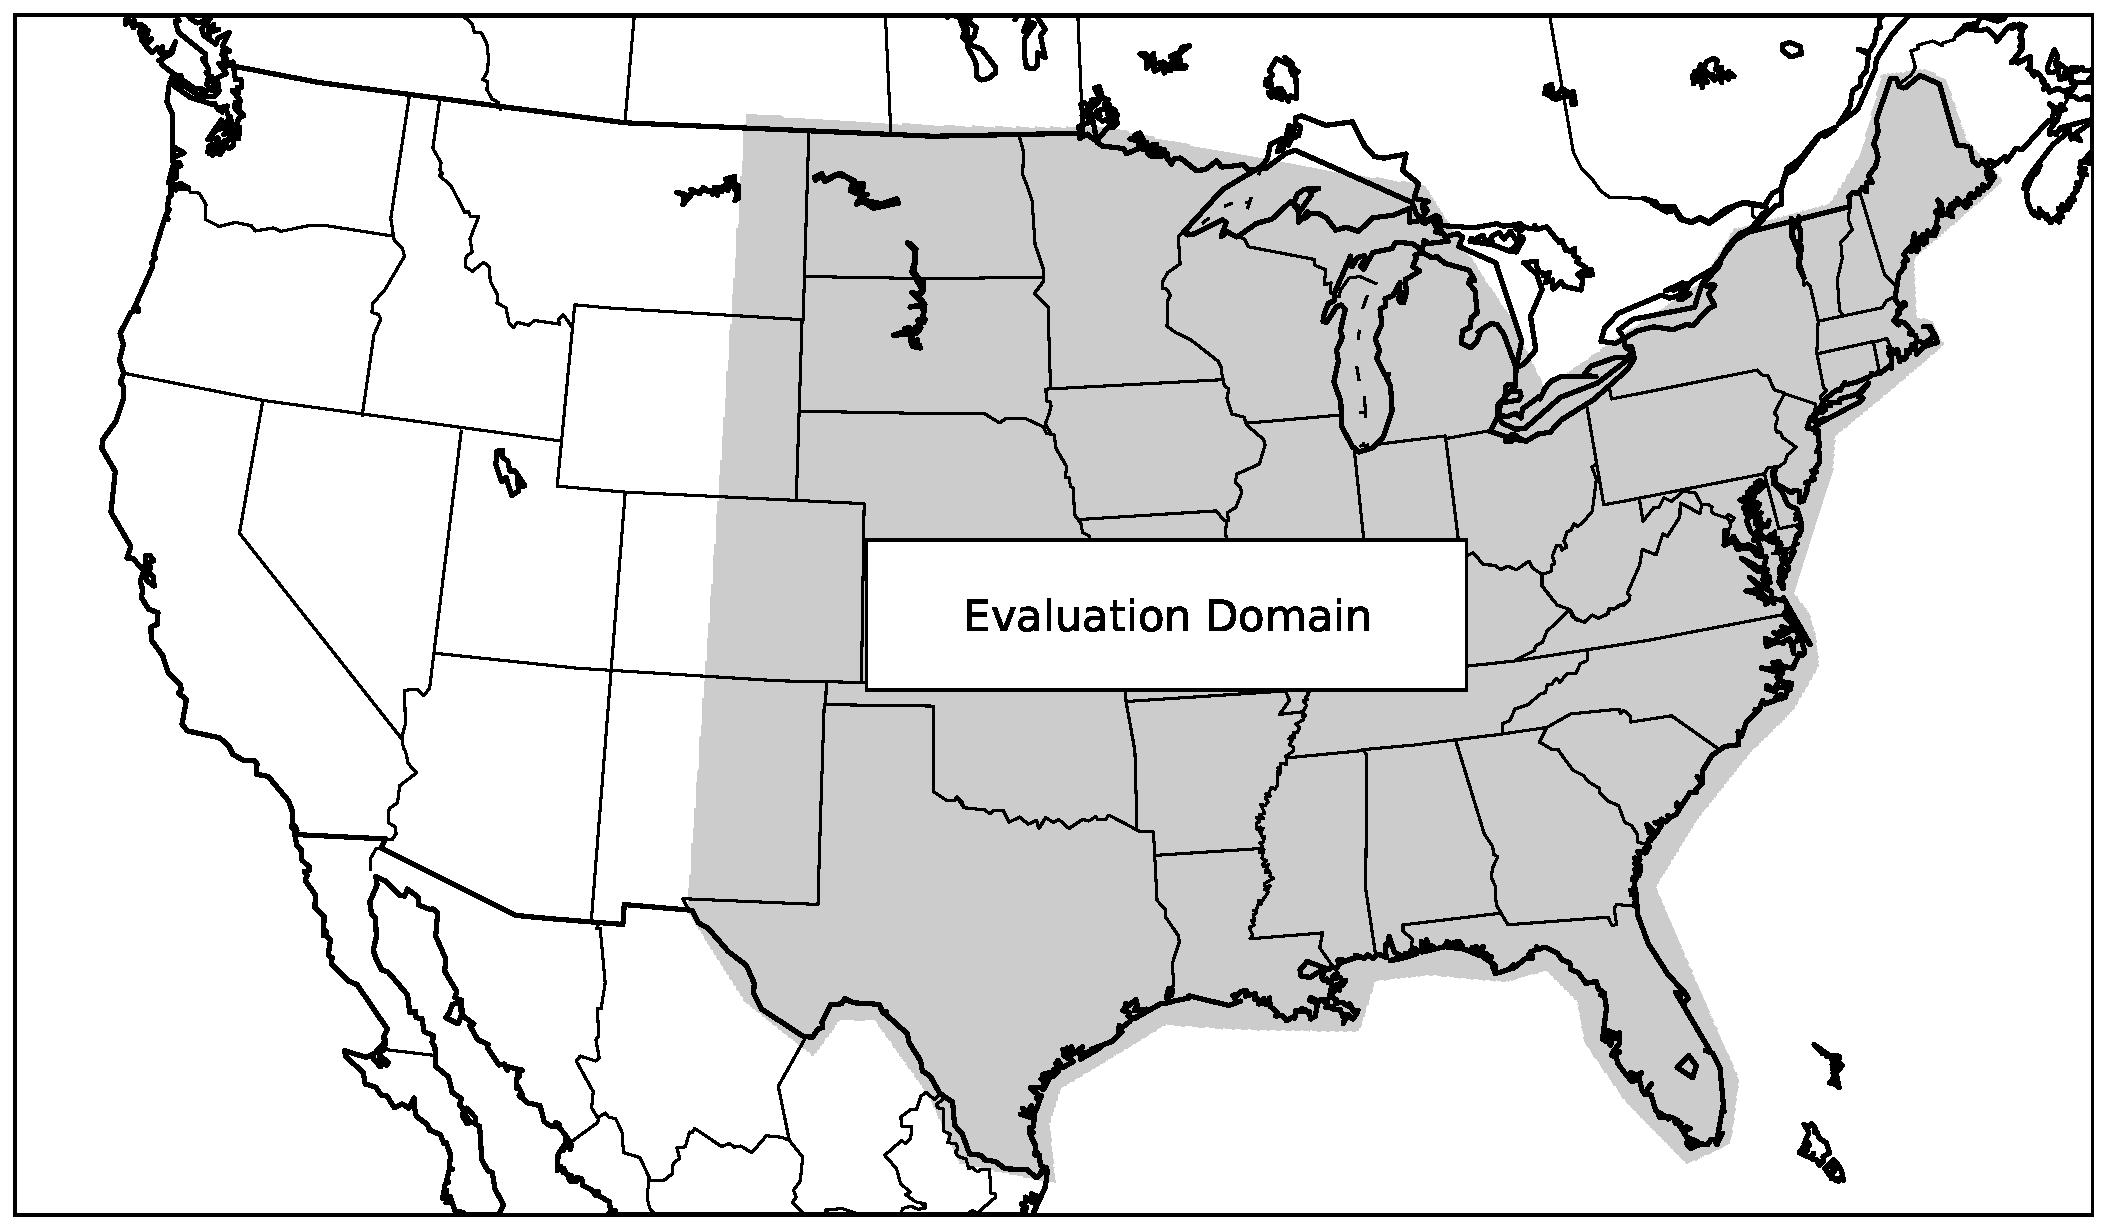
\includegraphics[width=35pc, angle=0]{./deterministic_data/domain.pdf}\\
    \caption{The subset of the Stage IV grid used in the analysis.}
    \label{domain}
\end{figure}
